\section{Переход к новому базису}
Для того, чтобы воспользоваться симплектическим методом нужно представить
Гамильтониан в виде:

\begin{equation} \label{nrk:eq:ham}
    \begin{cases}
        \dot{q_i} = \dfrac{\partial H}{\partial p_i}\\
        \dot{p_i} = -\dfrac{\partial H}{\partial q_i}
    \end{cases}
\end{equation}

Для этого в каждом состоянии системы для каждого атома введем пару базисных
векторов ($\bar e_{p_i}$ и $\bar e_{q_i}$) в касательной плоскости,
к единичной сфере с центром в координате атома,
в точке пересечения сферы и луча, пущенного из центра сферы в направлении спина
атома ($\bar s_i$).

\begin{figure}[h]\label{nrk:pic:basis}
    \centering
    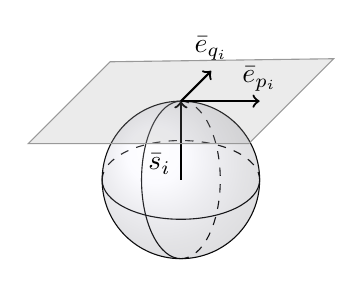
\begin{tikzpicture}
        \draw (-1,0) arc (180:360:1cm and 0.5cm);
        \draw[dashed] (-1,0) arc (180:0:1cm and 0.5cm);
        \draw (0,1) arc (90:270:0.5cm and 1cm);
        \draw[dashed] (0,1) arc (90:-90:0.5cm and 1cm);
        \draw (0,0) circle (1cm);
        \shade[ball color=blue!10!white,opacity=0.20] (0,0) circle (1cm);
        \draw[->, thick] (0,0) -- (0,1) node[left, pos=0.2]{$\bar s_i$};

        \filldraw[black!40, fill=black!40, fill opacity=0.2]
            (-1.4, 1, 1.4) --
            (-1.4, 1, -1.3) --
            (1.4, 1, -1.4) --
            (1.4, 1, 1.4) --
            cycle;

        \draw[->, thick] (0, 1, 0) -- (1, 1, 0) node[above]{$\bar e_{p_i}$};
        \draw[->, thick] (0, 1, 0) -- (0, 1, -1) node[above]{$\bar e_{q_i}$};
    \end{tikzpicture}
    \caption{Введение базисных векторов}
\end{figure}
